\documentclass[a4paper,landscape]{scrartcl}
\usepackage{fancybox}
\usepackage{tikz}
\usepackage{listings}
\usepackage[makeroom]{cancel}
\pagenumbering{gobble}
\renewcommand\CancelColor{\color{red}}
\usepackage{xcolor}
\lstset{escapeinside={<@}{@>}}

%\title{MergeSort-RecursionTree}
%\author{Manuel Kirsch}
%\date{}
\begin{document}
%    \ovalbox{
%    \begin{center}
    \begin{figure}
        \centering
        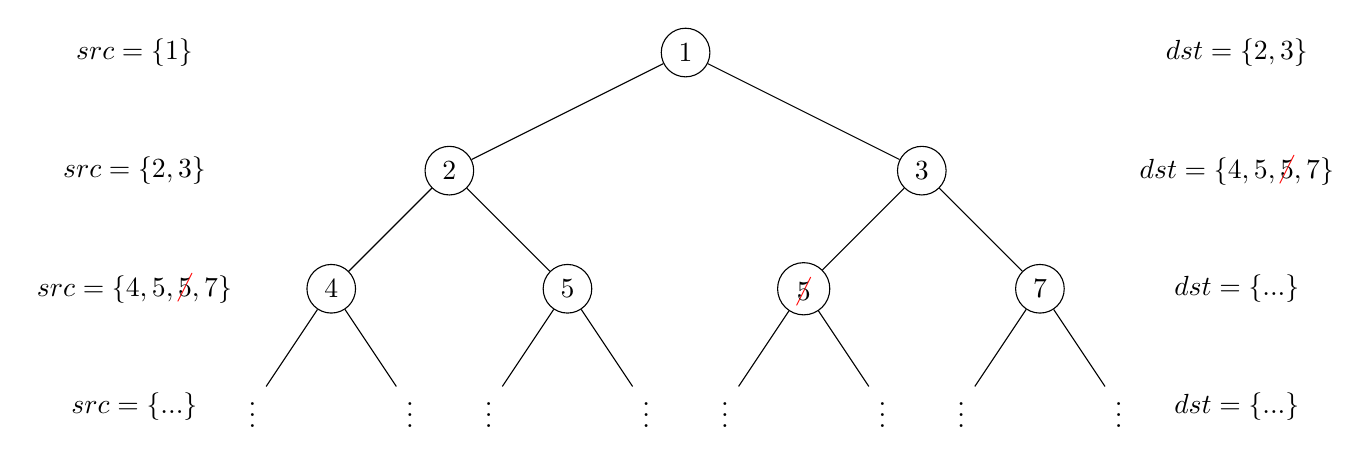
\begin{tikzpicture}[level/.style={sibling distance=60mm/#1}]
            \node [circle,draw] (z){$1$}
            child {node [circle,draw] (a) {$2$}
            child {node [circle,draw] (b) {$4$}
            child {node {$\vdots$}
            child [grow=left] {node (q) {$src = \{...\}$} edge from parent[draw=none]
            child [grow=up] {node (q) {$src = \{4,5,\cancel{5},7\}$} edge from parent[draw=none]
            child [grow=up] {node (q) {$src = \{2,3\}$} edge from parent[draw=none]
            child [grow=up] {node (q) {$src = \{1\}$} edge from parent[draw=none]}
            }
            }
            }
            }
            child {node {$\vdots$}}
            }
            child {node [circle,draw] (b) {$5$}
            child {node {$\vdots$}}
            child {node {$\vdots$}}
            }
            }
            child {node [circle,draw] (j) {$3$}
            child {node [circle,draw] (k) {$\cancel{5}$}
            child {node {$\vdots$}}
            child {node {$\vdots$}}
            }
            child {node [circle,draw] (l) {$7$}
            child {node {$\vdots$}}
            child {node {$\vdots$}
            child [grow=right] {node (q) {$dst = \{...\}$} edge from parent[draw=none]
            child [grow=up] {node (q) {$dst = \{...\}$} edge from parent[draw=none]
            child [grow=up] {node (r) {$dst = \{4,5,\cancel{5},7\}$ } edge from parent[draw=none]
            child [grow=up] {node (u) {$dst = \{2,3\}$ } edge from parent[draw=none]}
            }
            }}}
            }
            };
        \end{tikzpicture}
        %}

        \begin{lstlisting}[language=SQL,frame=single]
            SELECT <@\textcolor{red}{DISTINCT(dst)}@> FROM team22.relation_facebook WHERE src IN(
                SELECT <@\textcolor{red}{DISTINCT(dst)}@> FROM team22.relation_facebook WHERE src IN(
                    SELECT <@\textcolor{red}{DISTINCT(dst)}@> FROM team22.relation_facebook WHERE src IN(1)
                )
            )
        \end{lstlisting}
        \begin{lstlisting}[language=SQL,frame=single]
            SELECT <@\textcolor{red}{DISTINCT(rf3.dst)}@>
            FROM public.relation_facebook rf1,
            public.relation_facebook rf2,
            public.relation_facebook rf3
            WHERE rf2.src = rf1.dst
            AND rf3.src = rf2.dst
            AND rf1.src = 765;
        \end{lstlisting}
    \end{figure}


%    \end{center}

\end{document}